\documentclass[10pt,conference]{IEEEtran}

\usepackage{amsmath,amssymb,amsfonts}
\usepackage{booktabs}
\usepackage{graphicx}
\usepackage{cite}
\usepackage[hidelinks]{hyperref}

\graphicspath{{figures/}}

\newcommand{\PH}{ProtoHedge}
\newcommand{\DeepH}{Deep Hedging}
\newcommand{\OCE}{\mathrm{OCE}}

\begin{document}

\title{ProtoHedge Beyond Simulation: Empirical Validation on Historical Option Data}

\author{\IEEEauthorblockN{Yanis Zaim}
\IEEEauthorblockA{\textit{Columbia University}\\
New York, NY, USA\\
ymz2108@columbia.edu}
\and
\IEEEauthorblockN{Sayak Chakrabarty}
\IEEEauthorblockA{\textit{Northwestern University}\\
Evanston, IL, USA\\
sayak.chakrabarty@northwestern.edu}
\and
\IEEEauthorblockN{Imon Banerjee}
\IEEEauthorblockA{\textit{Northwestern University}\\
Evanston, IL, USA\\
imon.banerjee@northwestern.edu}
}

\maketitle

\begin{abstract}
Deep Hedging can learn effective risk-sensitive trading policies, but its
individual decisions are difficult to interpret. ProtoHedge addresses this
limitation by expressing each hedge as a similarity-weighted combination of
representative market states, providing an exact example-based decomposition while
retaining end-to-end learning. Existing evidence for the method is largely
simulation based, leaving its behavior in historical markets unresolved. We
conduct a controlled empirical evaluation of ProtoHedge against Deep Hedging
and a transparent delta-based benchmark across 34,395 historical option
episodes from ten U.S. underlyings and both standard and path-dependent option
liabilities. Under matched data, information, objectives, and evaluation
procedures, ProtoHedge remains competitive with Deep Hedging for European options and shows
encouraging tail-risk performance for path-dependent options, while comparing
favorably with the delta benchmark. These findings extend the evidence for
prototype-based hedging beyond simulation and suggest that interpretable policy
structure can retain competitive empirical performance on historical markets.
\end{abstract}

\begin{IEEEkeywords}
deep hedging, interpretable machine learning, option hedging, ProtoHedge,
conditional value-at-risk, sequential decision making
\end{IEEEkeywords}

\section{Introduction}

Hedging is a sequential decision problem under uncertainty. At each trading
date, a hedger must act from incomplete market information, absorb transaction
costs, respect position limits, and control a terminal loss distribution.
Deep Hedging (DH) addresses this problem by optimizing a neural policy directly
against a monetary utility objective \cite{buehler2019deep}. This formulation
can incorporate market frictions and complex state variables without requiring
a closed-form hedge. At each rebalancing date, the network maps observable
market conditions and current inventory to a trade; training over complete
paths balances terminal risk against cumulative transaction costs. Its
flexibility comes at a cost: the reason for an individual neural-network action
can be difficult to inspect.

ProtoHedge (PH) was proposed as an intrinsically interpretable alternative
\cite{faloughi2025protohedge}. PH retains DH's objective and sequential setup but
replaces its direct action map with a fixed library of representative market
states. Each trade is a similarity-weighted combination of actions attached to
those prototypes, so the examples and weights that generate a decision can be
retrieved exactly. The original PH experiments found near parity with DH in
Black--Scholes and stochastic-volatility simulators. The practical question is
whether this performance--interpretability tradeoff survives historical data,
where regimes change, option contracts expire, quotes are noisy, and nearby
rolling trajectories are dependent.

Prior work has evaluated neural and reinforcement-learning hedges under richer
simulators \cite{gao2023deeper,cao2021deep,kolm2019dynamic} and historical index
option data \cite{mikkila2023empirical,ruf2022hedging}. Our study asks a more
specific question: when DH and PH receive the same historical state, trade the
same instruments, and optimize the same tail-sensitive objective, does the PH
prototype bottleneck retain competitive out-of-sample performance? We evaluate
PH as a historical hedging model rather than as a test of any particular market
simulator.

Historical validation requires choices that are largely absent with independent
simulated paths. A listed option must remain the same contract throughout an
episode; windows must be formed after chronological splitting; the policy must
observe enough state to hedge a path-dependent payoff; and overlapping test
episodes require dependence-aware inference. Model and checkpoint selection
must also use validation data only. These choices determine what the comparison
means and are therefore part of the experimental contribution.

We make three contributions. First, we construct a contract-consistent
historical panel for ten liquid U.S. underlyings, with fixed 20-decision
horizons and a held-out 2022--2024 test period. Second, we compare DH with a
validation-selected PH family for both European and arithmetic-average Asian
calls under the original OCE CVaR@50\% utility. Third, we report paired
circular-block intervals, use validation-only checkpoint selection, and compare
PH directly with a transparent Spot-Delta rule. Under this protocol, PH is near
parity with DH for European calls, while the validation-tail-selected PH policy
has positive panel-level test utility relative to DH for Asian calls.

The experiments address three empirical questions. \emph{Q1:} Does replacing
DH's direct action head with the PH prototype bottleneck cause a detectable loss
of OCE utility for terminal-payoff European calls? The original simulation
evidence suggests that any loss should be small. \emph{Q2:} Does that conclusion
extend to arithmetic-average Asian liabilities, whose relevant state includes
the realized path? \emph{Q3:} Are conclusions robust to a transparent
market-delta benchmark and to temporal dependence among overlapping episodes?
We evaluate these questions on chronologically held-out paths and use paired
intervals that account for overlapping episodes, allowing us to distinguish
panel-wide evidence from rankings based only on average scores. The European
experiment transfers the original PH--DH comparison to historical data, while
the Asian experiment extends it to a liability whose payoff depends on the
realized path. Upon acceptance, we will release the source code, locked
configurations, data-construction scripts, and redistributable result artifacts
needed to reproduce the study. The underlying OptionMetrics and CRSP records
cannot be redistributed because they are proprietary and remain subject to
their providers' licenses.

\section{Related Work}

Classical delta hedging derives trades from model sensitivities
\cite{black1973pricing}. It is a local, model-based rule: the
position is determined by the option value's instantaneous response to the
underlying, rather than by direct optimization of the full distribution of
terminal hedging outcomes. Transaction costs and discrete rebalancing motivate
cost-sensitive policies \cite{leland1985transactions,whalley1997}. DH instead
learns the entire sequence of trades under a terminal risk objective, allowing
frictions, position constraints, and nonlinear risk preferences to enter the
training problem directly \cite{buehler2019deep}. Reinforcement-learning and
historical studies further demonstrate that neural hedging policies can be
trained and evaluated on observed option data
\cite{cao2021deep,mikkila2023empirical}; broader evidence is reviewed in
\cite{ruf2020review}.

PH brings prototype-based, case-based reasoning
\cite{li2018prototypes,chen2019looks} to DH \cite{faloughi2025protohedge}.
Prototype models are intrinsically interpretable in the sense that their output
is constructed from representative cases, rather than explained only after a
separate opaque model has made its prediction \cite{rudin2019stop}. PH applies
this idea at every rebalancing date by combining actions attached to
representative market states according to their similarity to the current
state. The resulting decomposition exposes the retrieved states, similarity
weights, and prototype actions behind each trade. The original study reports PH
competitive with DH in controlled simulations, suggesting that this
interpretable action bottleneck need not impose a large loss in hedging utility.

The literature therefore leaves a specific comparison unresolved: historical
studies validate DH, and simulation studies validate PH, but neither tests PH
against DH on historical paths. We match episodes, information, instruments,
the objective, and validation rules to test whether PH's
interpretability--performance tradeoff survives historical markets.

\section{Methods}

\subsection{Hedging Objective and Policies}

For hedge prices $P_t$, post-trade inventory $h_t$, trade increment $a_t$, and
terminal short-liability cash flow $H\leq0$, define
\begin{equation}
 O^\pi=H+\sum_{t=0}^{T-1}h_t^\top(P_{t+1}-P_t)
       -\sum_{t=0}^{T-1}\kappa_t^\top|a_t| .
 \label{eq:offset}
\end{equation}
We call $O^\pi$ the \emph{hedging offset} because it excludes the unobserved
premium of the synthetic liability. Higher values mean that a strategy offsets
more of the common terminal liability after transaction costs. Because all
policies face the same liability paths, paired differences isolate hedging
performance under this accounting convention.

Both neural policies use the same optimized certainty equivalent (OCE):
\begin{equation}
 \mathcal U_\lambda(O)=\sup_{y\in\mathbb R}
 \mathbb E[(1+\lambda)\min(O+y,0)-y],
 \label{eq:oce}
\end{equation}
with $\lambda=1$, corresponding to the lower 50\% tail used by the original
implementation \cite{bental2007oce,rockafellar2000}. We evaluate each trained
model with its frozen learned threshold $y$ and call the resulting mean
pathwise contribution \emph{OCE CVaR@50\% utility}. Higher values are better.

DH implements the trade $a_t$ with a feed-forward neural policy. PH instead
standardizes the current state $x_t$, maps it and fixed prototype states $p_k$
through a shared learned projection $f_\phi$, and sets
\begin{equation}
 \alpha_{t,k}=\frac{e^{-\lVert f_\phi(x_t)-f_\phi(p_k)\rVert^2}}
 {\sum_j e^{-\lVert f_\phi(x_t)-f_\phi(p_j)\rVert^2}},\qquad
 a_t=\sum_{k=1}^{K}\alpha_{t,k}b_k,
 \label{eq:proto}
\end{equation}
where $b_k$ is the learned bounded action of prototype $k$. The weights and
attached actions are the policy computation itself rather than a post-hoc
approximation. We therefore use \emph{inspectable} in the structural sense that
each proposed trade has an exact, model-native decomposition. Any subsequent
position-limit clipping is a shared deterministic feasibility step. The
empirical study tests whether a policy with this structure can remain
competitive in utility; whether the resulting explanations improve human
decisions requires a separate study.

\subsection{Historical Panel}

We combine OptionMetrics IvyDB US listed-option records with CRSP underlying
prices \cite{wrdsOptionMetrics,crspStock}. The underlyings are AAPL, IWM, NVDA,
QQQ, SPY, TLT, XLE, XLF, XLK, and XLV. They include two single stocks, broad
and sector equity exchange-traded funds, and a Treasury exchange-traded fund
over 2005--2024. This mix tests the same hedging protocol across idiosyncratic
equities, diversified portfolios, sector exposures, and an interest-rate-sensitive
asset rather than within a single market segment.

The quote screens ensure that both the policy state and friction proxy are
defined from usable observations. Retained records are American-style calls
with finite implied volatility and vendor Greeks, positive bids and midquotes,
and non-crossed offers. At each candidate start date, initial open interest must
be positive, relative spread cannot exceed one, and absolute strike moneyness
cannot exceed 10\%. This removes internally inconsistent or extremely illiquid
quotes before any model is trained.

Among surviving calls with 20--40 calendar days to expiration, contracts are
ranked by strike distance from spot, distance from a 30-day target maturity,
relative spread, open interest, and volume. The ranking uses no subsequent
hedging outcome. Once selected, the contract is held fixed: all 21 observations
must share its option identifier, strike, and expiration, and expiration must
follow the episode. Gaps longer than four calendar days begin a new block.
Requiring a complete fixed-contract path sacrifices sample size but prevents an
implicit daily roll between unrelated options, so each episode represents one
well-defined sequential hedging problem.

To preserve temporal order, we split the calendar before constructing rolling
windows. Training ends in 2018, validation covers 2019--2021, and testing covers
2022--2024. A 20-observation embargo at both post-training boundaries ensures
that no episode crosses a split or shares its horizon across that boundary.
Thus, model selection precedes the test period and each test episode represents
a later market path. The result is 20,537 training, 6,881 validation, and 6,977
test episodes, or 34,395 total (Table~\ref{tab:protocol}). Episodes may still
overlap within a period; the inference procedure accounts for that dependence.

\begin{table}[t]
\caption{Historical panel and locked protocol.}
\label{tab:protocol}
\centering
\footnotesize
\begin{tabular}{@{}ll@{}}
\toprule
Component & Specification \\
\midrule
Underlyings & AAPL, IWM, NVDA, QQQ, SPY, TLT, \\
 & XLE, XLF, XLK, XLV \\
Periods & Train through 2018; validation 2019--2021; \\
 & test 2022--2024; 20-observation embargo \\
Episodes & 20,537 train; 6,881 validation; 6,977 test \\
Episode unit & One option ID; 21 marks; 20 decisions \\
Liabilities & ATM European and arithmetic-average Asian calls \\
Hedge assets & Underlying and one fixed listed call \\
Neural runs & Three seeds; 800 epochs; common OCE objective \\
Inference & 2,000 paired circular-block draws; block length 20 \\
\bottomrule
\end{tabular}
\end{table}

Each episode defines a synthetic at-the-money short call struck at initial
spot $K_i=S_{i,0}$. The European payoff is
$H_i=-\max(S_{i,T}-K_i,0)$. The Asian payoff replaces terminal spot with the
arithmetic mean of the 20 end-of-interval fixings
\cite{kemna1990asian}. This pair contrasts a terminal-state liability with one
whose value depends on the realized path. The hedge instruments are the
underlying and the fixed listed call; trade increments and cumulative positions
are constrained to $[-1,1]$ for both.

The market record contains
$(S_t,C_t,\Delta_t,\nu_t,\sigma_t^{\mathrm{impl}})$: underlying spot,
fixed-option midpoint, vendor delta, vendor vega, and implied volatility. The
policy state is narrower: the networks receive current spot and option prices,
the two inventory positions, and time remaining; Asian policies additionally
receive running-average moneyness. Spot, option price, and vega are scaled
pathwise by initial spot. Variables outside the policy state still serve defined
protocol roles: vendor delta constructs Spot-Delta, delta, vega, and midpoint
construct option costs, and implied volatility supports screening. The running
average uses only fixings observed by the decision time. DH, every PH candidate,
and prototype extraction therefore receive the same task-appropriate inputs
without future path information.

Accounting is also common. The trade at time $t$ first updates cumulative
inventory, and that post-trade inventory earns the price change from $t$ to
$t+1$ in \eqref{eq:offset}. Applying only the latest trade increment to that
gain would incorrectly discard positions established earlier in the episode.
The short liability is settled only at the horizon.

Costs follow the original study's deterministic friction proxy. A stock trade
costs $0.0002|S_t|$ per unit; an option trade costs
$0.02|\nu_t|+0.0002|\Delta_t|+0.0005|C_t|$, using vendor vega $\nu_t$, delta
$\Delta_t$, and midpoint $C_t$. These stylized costs provide a common friction
model for the controlled policy comparison; every policy receives identical
prices and costs.

\subsection{Models and Baselines}

The transparent baseline, Spot-Delta, holds the selected listed call's observed
delta in the underlying and no option inventory. Because the signal is the
vendor delta of the listed hedge option, Spot-Delta is a market-based reference
rather than an analytical hedge for the synthetic liability. DH uses the
original paper-style feed-forward architecture with width 20, depth 3, and
Softplus activations.

PH uses $K\in\{10,25,50,100\}$ prototypes obtained by $K$-means
\cite{macqueen1967} from either DH or Spot-Delta training trajectories, with
unweighted or time-weighted similarity. Each centroid is replaced by its
nearest observed training state, preserving a concrete historical example.
Prototype anchors remain fixed while the projection and prototype actions are
learned. The two sources, two weighting rules, and four values of $K$ yield 16
PH configurations. DH-sourced, unweighted candidates are closest to the
original PH construction; Spot-Delta sourcing and time weighting extend it.

Two additional rules provide descriptive context in the archived outputs. An
unhedged strategy never trades. A no-trade-band delta rule retains its current
spot position while it lies inside a validation-tuned band around observed
delta and otherwise moves to the nearest edge. The primary comparisons use DH
and Spot-Delta as the neural and transparent benchmarks, respectively.

\subsection{Model and Checkpoint Selection}

Every neural policy uses three seeds, an 800-epoch budget, Adam with learning
rate $10^{-3}$, and the objective in \eqref{eq:oce}. Training also includes mean
absolute-action and inventory penalties of 0.001 and 0.002. These regularizers
stabilize optimization but are excluded from the test utility in
Table~\ref{tab:results}.

Within each ticker and liability, validation metrics are averaged across seeds.
\emph{Validation-Mean} selects the PH configuration with the highest mean
hedging offset, whereas \emph{Validation-Tail} selects the configuration with
the highest empirical CVaR@5\%. Candidates whose seed-averaged validation bound
occupancy exceeds 0.5 are screened out. Ties are resolved deterministically by
the alternate validation metric, lower occupancy, smaller $K$, and model name.
The resulting configuration is frozen before test evaluation.

PH searches 16 configurations per seed, whereas DH uses one fixed architecture.
Accordingly, our estimand is the performance of a validation-selected expanded
PH family against the original paper-style DH benchmark, not against an equally
tuned DH family. This distinction guards against overinterpreting family-level
model selection \cite{cawley2010overfitting}.

The initial checkpoint rule ranked saved epochs using validation OCE together
with small action, inventory, and bound-occupancy penalties. An audit found that
this rule selected the initialized DH policy in 12 of 60 fits. Although
initialization is an eligible checkpoint, the pattern showed that diagnostic
penalties could override improvement in the primary utility and made the
European comparison sensitive to the checkpoint criterion.

We therefore report a target-aligned sensitivity analysis. For the affected DH
fits and their matched selected PH candidates, the replacement checkpoint is
the one that maximizes validation OCE in the existing training history. This
requires no retraining: selection uses stored validation trajectories alone,
after which checkpoints are frozen for test evaluation. The original
penalized-score results remain archived to document the sensitivity.

\subsection{Statistical Inference}

For PH--DH comparisons, the primary statistic is the paired difference in
frozen-threshold OCE utility. For PH--Spot-Delta comparisons, we report mean
hedging offset and empirical CVaR@50\%. For each episode, neural-policy outcomes
are first averaged across seeds. We then resample paired episodes within each
ticker using 2,000 circular-block draws of length 20 and average the ten ticker
effects with equal weight \cite{politis1992,lahiri2003resampling}. Positive
differences favor PH; reported 95\% intervals are bootstrap percentile
intervals without multiplicity adjustment.

The resampling design targets an equal-asset effect. Seed averaging prevents a
historical episode from being counted three times, paired resampling compares
policies on the same paths, and equal ticker weights prevent larger panels from
dominating. The block length equals the full 20-decision horizon, preserving
dependence induced by strongly overlapping neighboring episodes.

\subsection{Empirical Estimand}

The primary estimand is the equal-asset, held-out PH--DH OCE effect produced by
each frozen validation rule, rather than the best test result available in the
grid. It therefore evaluates a deployable model-selection procedure instead of
rewarding a larger candidate family for an ex post test maximum. ``Tail'' names
the validation criterion; both selected policies are tested on the same OCE
utility.

OCE CVaR@50\% is primary because it is optimized by both architectures and is
the utility used to motivate PH. Mean hedging offset and empirical CVaR@50\%
against Spot-Delta provide complementary distributional summaries. RMSE,
downside deviation, trading cost, action magnitude, and bound occupancy are
archived as diagnostics rather than treated as additional headline tests.

PH is competitive when it retains its exact prototype decomposition without a
detectable loss under the primary utility. A positive interval supplies evidence
of improvement; an interval crossing zero supports only the weaker conclusion
that this study does not detect a difference.

\section{Results}

\subsection{Panel-Level Comparisons}

Table~\ref{tab:results} contains the primary ten-ticker results. Against DH,
the mean-selected European policy produces a PH difference of $+0.001009$, and
the tail-selected European policy produces $+0.000514$. Both intervals in
Table~\ref{tab:results} include zero. The data therefore support near parity,
not European PH superiority.

For Asian calls, Validation-Mean is positive but uncertain at $+0.001859$.
Validation-Tail is $+0.004015$, and its interval excludes zero. This is the only
primary PH--DH interval separated from zero. The OCE-only checkpoint analysis reduces the initial
European estimates of $+0.008841$ and $+0.006693$ by approximately 89\% and
92\%, while changing the Asian tail estimate by only 3\%. Eleven checkpoint
replacements enter each European comparison but only one enters each Asian
comparison, explaining why the European result is more sensitive to the
selection rule.

\begin{table*}[t]
\caption{Equal-ticker historical effects on the held-out 2022--2024 test period. Differences are PH minus benchmark; higher is better. PH--DH rows use frozen-threshold OCE CVaR@50\% utility after the targeted checkpoint sensitivity. PH--Spot-Delta rows use the Validation-Tail PH policy.}
\label{tab:results}
\centering
\footnotesize
\begin{tabular}{@{}llllrr@{}}
\toprule
Benchmark & Liability & Selection & Metric & Difference & 95\% block interval \\
\midrule
DH & European & Validation-Mean & OCE utility & +0.001009 & $[-0.002777,+0.005364]$ \\
DH & European & Validation-Tail & OCE utility & +0.000514 & $[-0.003418,+0.004734]$ \\
DH & Asian & Validation-Mean & OCE utility & +0.001859 & $[-0.000309,+0.003863]$ \\
DH & Asian & Validation-Tail & OCE utility & \textbf{+0.004015} & $\mathbf{[+0.001925,+0.006038]}$ \\
\midrule
Spot-Delta & European & Validation-Tail & Mean hedging offset & +0.005488 & $[+0.004086,+0.006858]$ \\
Spot-Delta & European & Validation-Tail & Empirical CVaR@50\% & +0.000163 & $[-0.001925,+0.002134]$ \\
Spot-Delta & Asian & Validation-Tail & Mean hedging offset & +0.002795 & $[+0.000271,+0.005291]$ \\
Spot-Delta & Asian & Validation-Tail & Empirical CVaR@50\% & \textbf{+0.005830} & $\mathbf{[+0.002925,+0.008393]}$ \\
\bottomrule
\end{tabular}
\end{table*}

The Spot-Delta comparisons provide a transparent second benchmark. European
Validation-Tail PH improves mean hedging offset by $0.005488$, but its empirical
CVaR@50\% difference is near zero. Asian Validation-Tail PH improves both mean
hedging offset ($+0.002795$) and empirical CVaR@50\% ($+0.005830$), with positive
intervals. Thus the Asian result is not solely an artifact of the DH benchmark,
although the OCE and empirical CVaR statistics should not be treated as
numerically interchangeable.

\subsection{Cross-Asset Evidence}

Fig.~\ref{fig:ticker-results} reports Validation-Tail PH--DH OCE differences
for every ticker. European effects are heterogeneous: four of ten estimates
are positive, only TLT has an interval wholly above zero, and no uniform
advantage is visible. Asian estimates are positive for seven of ten tickers;
AAPL, NVDA, TLT, and XLF have positive individual intervals, while no ticker
interval lies wholly below zero. Equal-ticker aggregation prevents large
underlyings or those with more windows from dominating the panel result.

\begin{figure*}[t]
\centering
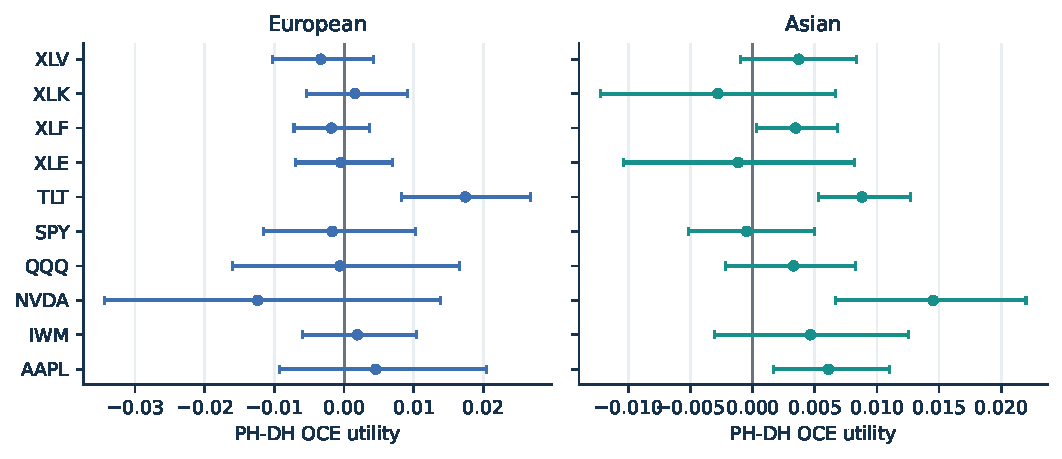
\includegraphics[width=0.88\textwidth]{audited_per_ticker_tail_cvar50.pdf}
\caption{Validation-Tail PH minus DH frozen-threshold OCE CVaR@50\% utility by ticker. Points are estimates and bars are paired 95\% circular-block intervals. Positive values favor PH.}
\label{fig:ticker-results}
\end{figure*}

The cross-asset pattern matters for interpretation. The positive Asian panel
effect is not produced by one asset, but neither is it universal. Its strongest
estimates occur for AAPL, NVDA, and TLT, while SPY is near zero and XLE and XLK
are negative with wide intervals. This heterogeneity supports a panel-level
path-dependent tail finding and motivates future regime analysis.

Validation-Mean does not change the panel conclusion. Seven of ten point
estimates are positive for each liability, but both equal-ticker intervals cross
zero. The supported Asian improvement is therefore specific to the
Validation-Tail selection rule rather than a general mean-performance advantage.

\subsection{Checkpoint Diagnostic}

Bound occupancy helps explain the checkpoint sensitivity. DH occupies an inventory
bound in approximately 39\% of test path--time--instrument observations for both
liabilities, whereas selected PH policies average roughly 4--5\% for European
and 2\% for Asian calls. Because occupancy is a diagnostic rather than the test
objective, including it in the initial checkpoint score disproportionately
favored lower-occupancy policies. OCE-only selection aligns checkpoint choice
with the reported utility.

\section{Discussion}

The European result supports PH's original performance--interpretability
premise on historical data. Replacing the final black-box action map
with a prototype mixture does not produce a statistically detectable utility
loss across the ten-ticker panel. Near parity is meaningful here because PH
retains a direct, model-native decomposition of each proposed trade into
similarities and prototype actions.

The Asian result raises the study's main forward-looking hypothesis: routing
actions through a finite reference set may regularize a policy when the
liability state depends on the path. Both models receive the same
running-average moneyness state, but the prototype bottleneck constrains how PH
turns that information into trades. The present experiment cannot separate
this mechanism from PH's larger configuration search. It nevertheless
identifies path-dependent tail hedging as a promising setting for a matched,
independently confirmed comparison.

The benchmarks answer complementary questions. DH largely isolates the effect
of the prototype action bottleneck, whereas Spot-Delta anchors the evaluation
to a transparent rule independent of neural training. The Asian advantage
appears against both; the European evidence supports competitiveness but not a
tail improvement. This agreement strengthens the Asian signal without removing
the need for a matched-search confirmation.

\subsection{Limitations and Next Steps}

\emph{Model selection.} PH receives a larger development budget than the fixed
DH benchmark, and 25 of 40 selected configurations use an added prototype source
or similarity weighting. The evidence therefore applies to a
validation-selected PH family rather than one portable configuration. The
checkpoint analysis reuses stored training histories. A fully matched study
should equalize search budgets, use OCE checkpoint selection from the outset,
and lock one PH design across assets.

\emph{Market realism.} Daily midquotes and stylized costs provide a controlled
comparison but not an executable slippage model. The liability is synthetic and
at the money, while the hedge option is a selected listed contract. Because the
unobserved liability premium is omitted, absolute hedging-offset levels are
comparative rather than profitability measures. Further tests should add
maturity and moneyness buckets and executable spread models.

\emph{Generalization and inference.} Chronological testing measures transfer to
later regimes of the same ten underlyings, not to unseen assets. The evidence is
also limited to liquid U.S. names, one horizon, and call liabilities. Block
resampling preserves within-ticker temporal dependence but not synchronous
cross-ticker shocks, and the four PH--DH intervals are not multiplicity adjusted.
Independent confirmation should therefore include new assets and periods and a
panel-aware multiple-testing design.

\section{Reproducibility}

Our reproducibility archive preserves the locked historical protocol, SHA-256
manifests, outputs for all ticker--liability tasks and seeds, candidate and
checkpoint identities, pathwise paired outcomes, bootstrap results, and the
asset-generation script. Tables and figures are generated from archived CSV
files rather than transcribed manually. The original run remains immutable,
with the checkpoint sensitivity stored as a separate analysis. Upon acceptance,
we will release the code, configurations, data-construction scripts, and
redistributable artifacts; the underlying OptionMetrics and CRSP records remain
subject to their providers' licenses.

\section{Conclusion}

This study extends ProtoHedge from simulation to historical option markets
across ten U.S. underlyings and two liability structures. With validation-only
selection and paired temporal-block inference, PH remains competitive with DH
for European calls and preserves an exact prototype decomposition of each
proposed trade. For arithmetic-average Asian calls, the tail-selected PH family
yields a positive panel-level OCE utility difference against DH. It also
improves mean and empirical lower-tail outcomes against Spot-Delta.

These findings provide historical support for prototype-based hedging and
identify path-dependent liabilities as the most promising setting for further
study. A matched-search, fixed-configuration experiment should next test
whether the prototype bottleneck itself supplies useful regularization across
assets and market regimes. More broadly, the results suggest that interpretable
policy structure can remain compatible with risk-sensitive sequential decision
making in observed markets.

\section*{Acknowledgment}

The authors used OpenAI Codex \cite{openaiCodex2026} for software-development,
drafting, and language-editing assistance throughout all sections of this
manuscript. The authors independently reviewed and validated all generated code
and text, verified the analysis, citations, and claims, and take full
responsibility for the work.

\bibliographystyle{IEEEtran}
\bibliography{references_empirical}

\end{document}
